\protect\hyperlink{main-nav}{≡} \protect\hyperlink{close-nav}{×}

\hypertarget{section-1.1-functions}{%
\section{Section 1.1: Functions}\label{section-1.1-functions}}

\hypertarget{what-is-a-function}{%
\subsubsection{What is a function?}\label{what-is-a-function}}

The natural world is full of relationships between quantities that
change. When we see these relationships, it is natural for us to ask
``If I know one quantity, can I then determine the other?'' This
establishes the idea of an input quantity, or independent variable, and
a corresponding output quantity, or dependent variable. From this we get
the notion of a functional relationship in which the output can be
determined from the input.

For some quantities, like height and age, there are certainly
relationships between these quantities. Given a specific person and any
age, it is easy enough to determine their height, but if we tried to
reverse that relationship and determine height from a given age, that
would be problematic, since most people maintain the same height for
many years.

\hypertarget{function}{%
\paragraph{Function}\label{function}}

A \textbf{function} is rule for a relationship between an input, or
independent, quantity and an output, or dependent, quantity in which
each input value uniquely determines one output value. We say ``the
output is a function of the input.''

\hypertarget{example-1}{%
\paragraph{Example 1}\label{example-1}}

In the height and age example above, is height a function of age? Is age
a function of height?

In the height and age example above, it would be correct to say that
height is a function of age, since each age uniquely determines a
height. For example, on my 18th birthday, I had exactly one height of 69
inches.

However, age is not a function of height, since one height input might
correspond with more than one output age. For example, for an input
height of 70 inches, there is more than one output of age since I was 70
inches at the age of 20 and 21.

To view this video please enable JavaScript, and consider upgrading to a
web browser that \href{http://videojs.com/html5-video-support/}{supports
HTML5 video}

\hypertarget{function-notation}{%
\subsubsection{Function Notation}\label{function-notation}}

To simplify writing out expressions and equations involving functions, a
simplified notation is often used. We also use descriptive variables to
help us remember the meaning of the quantities in the problem.

Rather than write ``height is a function of age,'' we could use the
descriptive variable \textbackslash{}(h\textbackslash{}) to represent
height and we could use the descriptive variable
\textbackslash{}(a\textbackslash{}) to represent age.

\begin{longtable}[]{@{}ll@{}}
\toprule
\endhead
"height is a function of age" & if we name the function
\textbackslash{}(f\textbackslash{}) we write\tabularnewline
"\textbackslash{}(h\textbackslash{}) is
\textbackslash{}(f\textbackslash{}) of
\textbackslash{}(a\textbackslash{})" & or more simply\tabularnewline
\textbackslash{}(h = f(a)\textbackslash{}) & we could instead name the
function \textbackslash{}(h\textbackslash{}) and write\tabularnewline
\textbackslash{}(h(a)\textbackslash{}) & which is read
"\textbackslash{}(h\textbackslash{}) of
\textbackslash{}(a\textbackslash{})"\tabularnewline
\bottomrule
\end{longtable}

Remember we can use any variable to name the function; the notation
\textbackslash{}(h(a)\textbackslash{}) shows us that
\textbackslash{}(h\textbackslash{}) depends on
\textbackslash{}(a\textbackslash{}). The value
``\textbackslash{}(a\textbackslash{})'' must be put into the function
``\textbackslash{}(h\textbackslash{})'' to get a result. Be careful --
the parentheses indicate that age is input into the function (Note: do
not confuse these parentheses with multiplication!).

\hypertarget{function-notation-1}{%
\paragraph{Function Notation}\label{function-notation-1}}

The notation output = \textbackslash{}(f\textbackslash{})(input) defines
a function named \textbackslash{}(f\textbackslash{}). This would be read
``output is \textbackslash{}(f\textbackslash{}) of input.''

\hypertarget{example-2}{%
\paragraph{Example 2}\label{example-2}}

A function \textbackslash{}(N = f(y)\textbackslash{}) gives the number
of police officers, \textbackslash{}(N\textbackslash{}), in a town in
year \textbackslash{}(y\textbackslash{}). What does
\textbackslash{}(f(2005) = 300\textbackslash{}) tell us?

When we read \textbackslash{}(f(2005) = 300\textbackslash{}), we see the
input quantity is 2005, which is a value for the input quantity of the
function, the year (\textbackslash{}(y\textbackslash{})). The output
value is 300, the number of police officers
(\textbackslash{}(N\textbackslash{})), a value for the output quantity.
Remember \textbackslash{}(N=f(y)\textbackslash{}). So this tells us that
in the year 2005 there were 300 police officers in the town.

\hypertarget{tables-as-functions}{%
\subsubsection{Tables as Functions}\label{tables-as-functions}}

Functions can be represented in many ways: Words (as we did in the last
few examples), tables of values, graphs, or formulas. Represented as a
table, we are presented with a list of input and output values.

This table represents the age of children in years and their
corresponding heights. While some tables show all the information we
know about a function, this particular table represents just some of the
data available for height and ages of children.

\begin{longtable}[]{@{}llllllll@{}}
\toprule
\endhead
(input) \textbackslash{}(a\textbackslash{}), age in years & 4 & 5 & 6 &
7 & 8 & 9 & 10\tabularnewline
(output) \textbackslash{}(h\textbackslash{}), height in inches & 40 & 42
& 44 & 47 & 50 & 52 & 54\tabularnewline
\bottomrule
\end{longtable}

\hypertarget{example-3}{%
\paragraph{Example 3}\label{example-3}}

Which of these tables define a function (if any)?

\begin{longtable}[]{@{}ll@{}}
\toprule
\endhead
Input & Output\tabularnewline
2 & 1\tabularnewline
5 & 3\tabularnewline
8 & 6\tabularnewline
\bottomrule
\end{longtable}

\begin{longtable}[]{@{}ll@{}}
\toprule
\endhead
Input & Output\tabularnewline
-3 & 5\tabularnewline
0 & 1\tabularnewline
4 & 5\tabularnewline
\bottomrule
\end{longtable}

\begin{longtable}[]{@{}ll@{}}
\toprule
\endhead
Input & Output\tabularnewline
1 & 0\tabularnewline
5 & 2\tabularnewline
5 & 4\tabularnewline
\bottomrule
\end{longtable}

The first and second tables define functions. In both, each input
corresponds to exactly one output. The third table does not define a
function since the input value of 5 corresponds with two different
output values.

To view this video please enable JavaScript, and consider upgrading to a
web browser that \href{http://videojs.com/html5-video-support/}{supports
HTML5 video}

\hypertarget{solving-and-evaluating-functions}{%
\subsubsection{Solving and Evaluating
Functions}\label{solving-and-evaluating-functions}}

When we work with functions, there are two typical things we do:
evaluate and solve. Evaluating a function is what we do when we know an
input, and use the function to determine the corresponding output.
Evaluating will always produce one result, since each input of a
function corresponds to exactly one output.

Solving equations involving a function is what we do when we know an
output, and use the function to determine the inputs that would produce
that output. Solving a function could produce more than one solution,
since different inputs can produce the same output.

\hypertarget{example-4}{%
\paragraph{Example 4}\label{example-4}}

Using the table shown, where \textbackslash{}(Q=g(n)\textbackslash{})

\begin{longtable}[]{@{}llllll@{}}
\toprule
\endhead
\textbackslash{}(n\textbackslash{}) & 1 & 2 & 3 & 4 & 5\tabularnewline
\textbackslash{}(Q\textbackslash{}) & 8 & 6 & 7 & 6 & 8\tabularnewline
\bottomrule
\end{longtable}

a) Evaluate \textbackslash{}(g(3)\textbackslash{})\\
b) Solve \textbackslash{}(g(n)=6\textbackslash{})

a) Evaluate \textbackslash{}(g(3)\textbackslash{}): Evaluating
\textbackslash{}(g(3)\textbackslash{}) (read: ``g of 3'') means that we
need to determine the output value, \textbackslash{}(Q\textbackslash{}),
of the function g given the input value of
\textbackslash{}(n=3\textbackslash{}). Looking at the table, we see the
output corresponding to \textbackslash{}(n=3\textbackslash{}) is
\textbackslash{}(Q=7\textbackslash{}), allowing us to conclude
\textbackslash{}(g(3) = 7\textbackslash{}).

b) Solve \textbackslash{}(g(n)=6\textbackslash{}): Solving
\textbackslash{}(g(n) = 6\textbackslash{}) means we need to determine
what input values, \textbackslash{}(n\textbackslash{}), produce an
output value of 6. Looking at the table we see there are two solutions:
\textbackslash{}(n = 2\textbackslash{}) and \textbackslash{}(n =
4\textbackslash{}). When we input 2 into the function
\textbackslash{}(g\textbackslash{}), our output is \textbackslash{}(Q =
6\textbackslash{}). When we input 4 into the function
\textbackslash{}(g\textbackslash{}), our output is also
\textbackslash{}(Q = 6\textbackslash{}).

\hypertarget{graphs-as-functions}{%
\subsubsection{Graphs as Functions}\label{graphs-as-functions}}

Oftentimes a graph of a relationship can be used to define a function.
By convention, graphs are typically created with the input quantity
along the horizontal axis and the output quantity along the vertical.

\hypertarget{example-5}{%
\paragraph{Example 5}\label{example-5}}

Which of these graphs defines a function
\textbackslash{}(y=f(x)\textbackslash{})?

\begin{figure}
\centering
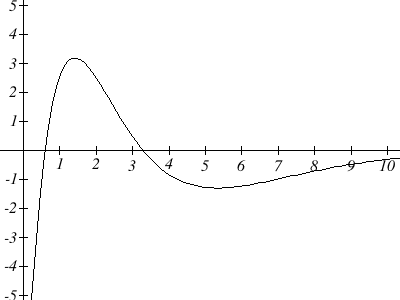
\includegraphics{images/image081.png}
\caption{}
\end{figure}

Looking at the three graphs above, the first two define a function
\textbackslash{}(y=f(x)\textbackslash{}), since for each input value
along the horizontal axis there is exactly one output value
corresponding, determined by the y-value of the graph. The third graph
does not define a function \textbackslash{}(y=f(x)\textbackslash{})
since some input values, such as \textbackslash{}(x=2\textbackslash{}),
correspond with more than one output value.

\hypertarget{vertical-line-test}{%
\paragraph{Vertical Line Test}\label{vertical-line-test}}

The \textbf{vertical line test} is a handy way to think about whether a
graph defines the vertical output as a function of the horizontal input.
Imagine drawing vertical lines through the graph. If any vertical line
would cross the graph more than once, then the graph does not define
only one vertical output for each horizontal input.

To view this video please enable JavaScript, and consider upgrading to a
web browser that \href{http://videojs.com/html5-video-support/}{supports
HTML5 video}

Evaluating a function using a graph requires taking the given input and
using the graph to look up the corresponding output. Solving a function
equation using a graph requires taking the given output and looking on
the graph to determine the corresponding input.

\hypertarget{example-6}{%
\paragraph{Example 6}\label{example-6}}

Given the graph below,

\begin{figure}
\centering
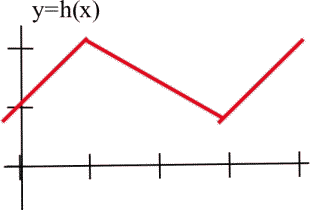
\includegraphics{images/image084.png}
\caption{}
\end{figure}

a) Evaluate \textbackslash{}(f(2)\textbackslash{}).\\
b) Solve \textbackslash{}(f(x) = 4\textbackslash{}).

a) To evaluate \textbackslash{}(f(2)\textbackslash{}), we find the input
of \textbackslash{}(x=2\textbackslash{}) on the horizontal axis. Moving
up to the graph gives the point (2, 1), giving an output of
\textbackslash{}(y=1\textbackslash{}). So \textbackslash{}(f(2) =
1\textbackslash{}).

b) To solve \textbackslash{}(f(x) = 4\textbackslash{}), we find the
value 4 on the vertical axis because if \textbackslash{}(f(x) =
4\textbackslash{}) then 4 is the output. Moving horizontally across the
graph gives two points with the output of 4: (-1,4) and (3,4). These
give the two solutions to \textbackslash{}(f(x) = 4\textbackslash{}):
\textbackslash{}(x = -1\textbackslash{}) or \textbackslash{}(x =
3\textbackslash{}). This means \textbackslash{}(f(-1)=4\textbackslash{})
and \textbackslash{}(f(3)=4\textbackslash{}), or when the input is -1 or
3, the output is 4.

Notice that while the graph in the previous example is a function,
getting two input values for the output value of 4 shows us that this
function is not one-to-one.

\hypertarget{formulas-as-functions}{%
\subsubsection{Formulas as Functions}\label{formulas-as-functions}}

When possible, it is very convenient to define relationships using
formulas. If it is possible to express the output as a formula involving
the input quantity, then we can define a function.

\hypertarget{example-7}{%
\paragraph{Example 7}\label{example-7}}

Express the relationship \textbackslash{}(2n + 6p = 12\textbackslash{})
as a function \textbackslash{}(p = f(n)\textbackslash{}) if possible.

To express the relationship in this form, we need to be able to write
the relationship where \textbackslash{}(p\textbackslash{}) is a function
of \textbackslash{}(n\textbackslash{}), which means writing it as
\textbackslash{}(p =\textbackslash{}) {[}something involving
\textbackslash{}(n\textbackslash{}){]}.

\begin{longtable}[]{@{}ll@{}}
\toprule
\endhead
\textbackslash{}(2n + 6p = 12\textbackslash{}) & subtract
\textbackslash{}(2n\textbackslash{}) from both sides\tabularnewline
\textbackslash{}(6p = 12 - 2n\textbackslash{}) & divide both sides by 6
and simplify\tabularnewline
\bottomrule
\end{longtable}

\textbackslash{}{[}p=\textbackslash{}frac\{12-2n\}\{6\}=\textbackslash{}frac\{12\}\{6\}-\textbackslash{}frac\{2n\}\{6\}=2-\textbackslash{}frac\{1\}\{3\}n\textbackslash{}{]}

Having rewritten the formula as \textbackslash{}(p=\textbackslash{}), we
can now express \textbackslash{}(p\textbackslash{}) as a function:
\textbackslash{}(p=f(n)=2-\textbackslash{}frac\{1\}\{3\}n\textbackslash{})

Not every relationship can be expressed as a function with a formula.

As with tables and graphs, it is common to evaluate and solve functions
involving formulas. Evaluating will require replacing the input variable
in the formula with the value provided and calculating. Solving will
require replacing the output variable in the formula with the value
provided, and solving for the input(s) that would produce that output.

\hypertarget{example-8}{%
\paragraph{Example 8}\label{example-8}}

Given the function \textbackslash{}(k(t)=t\^{}3+2\textbackslash{}):\\
a) Evaluate \textbackslash{}(k(2)\textbackslash{}).\\
b) Solve \textbackslash{}(k(t)=1\textbackslash{}).

a) To evaluate \textbackslash{}(k(2)\textbackslash{}), we plug in the
input value 2 into the formula wherever we see the input variable
\textbackslash{}(t\textbackslash{}), then simplify:
\textbackslash{}{[}\textbackslash{}begin\{align*\}k(2)=\&2\^{}3+2\textbackslash{}\textbackslash{}k(2)=\&8+2
\textbackslash{}end\{align*\}\textbackslash{}{]} So
\textbackslash{}(k(2) = 10\textbackslash{}).

b) To solve \textbackslash{}(k(t) = 1\textbackslash{}), we set the
formula for \textbackslash{}(k(t)\textbackslash{}) equal to 1, and solve
for the input value that will produce that output:
\textbackslash{}{[}\textbackslash{}begin\{align*\} k(t)=\&1 \&
\textbackslash{}\textbackslash{} t\^{}3+2=\&1
\&\textbackslash{}text\{substitute the original formula\}
\textbackslash{}\textbackslash{} t\^{}3=\&-1
\&\textbackslash{}text\{subtract 2 from each side\}
\textbackslash{}\textbackslash{} t=\&1 \&\textbackslash{}text\{take the
cube root of each side\}
\textbackslash{}end\{align*\}\textbackslash{}{]}

When solving an equation using formulas, you can check your answer by
using your solution in the original equation to see if your calculated
answer is correct.

We want to know if \textbackslash{}(k(t) = 1\textbackslash{}) is true
when \textbackslash{}(t=-1\textbackslash{}):
\textbackslash{}{[}\textbackslash{}begin\{align*\}k(-1)=\&(-1)\^{}3+2\textbackslash{}\textbackslash{}=\&
-1+2\textbackslash{}\textbackslash{}=\&1,\textbackslash{}end\{align*\}\textbackslash{}{]}
which was the desired result.

\hypertarget{basic-toolkit-functions}{%
\subsubsection{Basic Toolkit Functions}\label{basic-toolkit-functions}}

There are some basic functions that it is helpful to know the name and
shape of. We call these the basic ``toolkit of functions.'' For these
definitions we will use \textbackslash{}(x\textbackslash{}) as the input
variable and \textbackslash{}(f(x)\textbackslash{}) as the output
variable.

\hypertarget{toolkit-functions}{%
\paragraph{Toolkit Functions}\label{toolkit-functions}}

\begin{longtable}[]{@{}ll@{}}
\toprule
\endhead
Constant: & \textbackslash{}(f(x)=c\textbackslash{}), where
\textbackslash{}(c\textbackslash{}) is a constant
(number)\tabularnewline
Identity: & \textbackslash{}(f(x)=x\textbackslash{})\tabularnewline
Absolute Value: &
\textbackslash{}(f(x)=\textbar{}x\textbar{}\textbackslash{})\tabularnewline
Quadratic: &
\textbackslash{}(f(x)=x\^{}2\textbackslash{})\tabularnewline
Cubic: & \textbackslash{}(f(x)=x\^{}3\textbackslash{})\tabularnewline
Reciprocal: &
\textbackslash{}(f(x)=\textbackslash{}frac\{1\}\{x\}\textbackslash{})\tabularnewline
Reciprocal squared: &
\textbackslash{}(f(x)=\textbackslash{}frac\{1\}\{x\^{}2\}\textbackslash{})\tabularnewline
Square root: &
\textbackslash{}(f(x)=\textbackslash{}sqrt{[}2{]}\{x\}=\textbackslash{}sqrt\{x\}\textbackslash{})\tabularnewline
Cube root: &
\textbackslash{}(f(x)=\textbackslash{}sqrt{[}3{]}\{x\}\textbackslash{})\tabularnewline
\bottomrule
\end{longtable}

\hypertarget{graphs-of-the-toolkit-functions}{%
\subsubsection{Graphs of the Toolkit
Functions}\label{graphs-of-the-toolkit-functions}}

\begin{figure}
\centering
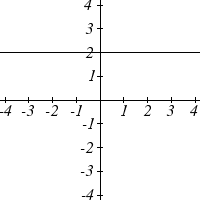
\includegraphics{images/image085.png}
\caption{Constant, \textbackslash{}(f(x)=c\textbackslash{}) (c is 2 in
this picture).}
\end{figure}

\begin{figure}
\centering
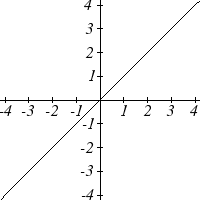
\includegraphics{images/image086.png}
\caption{Identity: \textbackslash{}(f(x)=x\textbackslash{}).}
\end{figure}

\begin{figure}
\centering
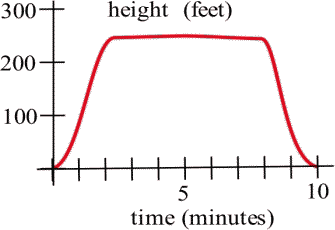
\includegraphics{images/image087.png}
\caption{Absolute Value:
\textbackslash{}(f(x)=\textbar{}x\textbar{}\textbackslash{})}
\end{figure}

\begin{figure}
\centering
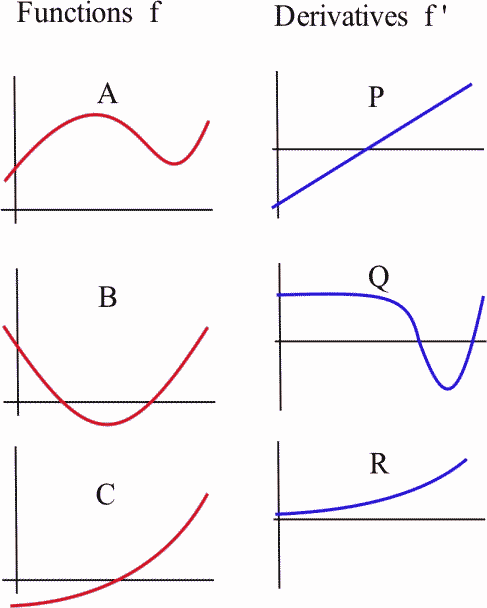
\includegraphics{images/image088.png}
\caption{Quadratic: \textbackslash{}(f(x)=x\^{}2\textbackslash{})}
\end{figure}

\begin{figure}
\centering
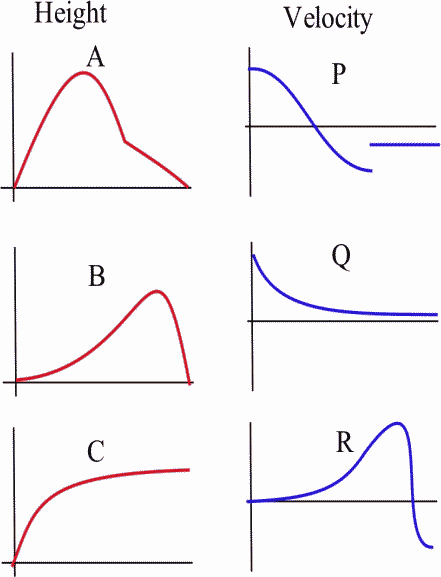
\includegraphics{images/image089.png}
\caption{Cubic: \textbackslash{}(f(x)=x\^{}3\textbackslash{})}
\end{figure}

\begin{figure}
\centering
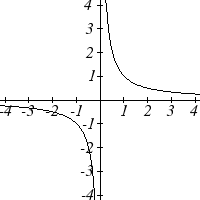
\includegraphics{images/image092.png}
\caption{Reciprocal:
\textbackslash{}(f(x)=\textbackslash{}frac\{1\}\{x\}\textbackslash{})}
\end{figure}

\begin{figure}
\centering
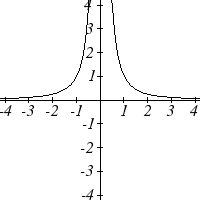
\includegraphics{images/image093.png}
\caption{Reciprocal squared:
\textbackslash{}(f(x)=\textbackslash{}frac\{1\}\{x\^{}2\}\textbackslash{})}
\end{figure}

\begin{figure}
\centering
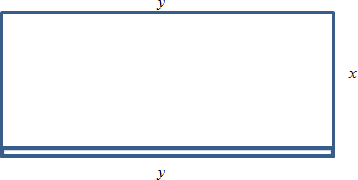
\includegraphics{images/image090.png}
\caption{Square root:
\textbackslash{}(f(x)=\textbackslash{}sqrt{[}2{]}\{x\}=\textbackslash{}sqrt\{x\}\textbackslash{})}
\end{figure}

\begin{figure}
\centering
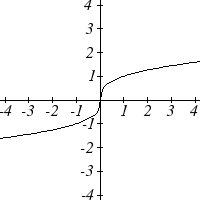
\includegraphics{images/image091.png}
\caption{Cube root:
\textbackslash{}(f(x)=\textbackslash{}sqrt{[}3{]}\{x\}\textbackslash{})}
\end{figure}

To view this video please enable JavaScript, and consider upgrading to a
web browser that \href{http://videojs.com/html5-video-support/}{supports
HTML5 video}

One of our main goals in mathematics is to model the real world with
mathematical functions. In doing so, it is important to keep in mind the
limitations of those models we create.

This table shows a relationship between circumference and height of a
tree as it grows.

\begin{longtable}[]{@{}llllll@{}}
\toprule
\endhead
Circumference, \textbackslash{}(c\textbackslash{}) & 1.7 & 2.5 & 5.5 &
8.2 & 13.7\tabularnewline
Height, \textbackslash{}(h\textbackslash{}) & 24.5 & 31 & 45.2 & 54.6 &
92.1\tabularnewline
\bottomrule
\end{longtable}

While there is a strong relationship between the two, it would certainly
be ridiculous to talk about a tree with a circumference of -3 feet, or a
height of 3000 feet. When we identify limitations on the inputs and
outputs of a function, we are determining the domain and range of the
function.

\hypertarget{domain-and-range}{%
\paragraph{Domain and Range}\label{domain-and-range}}

\textbf{Domain:} The set of possible input values to a function.\\
\textbf{Range:} The set of possible output values of a function

\hypertarget{example-9}{%
\paragraph{Example 9}\label{example-9}}

Using the tree table above, determine a reasonable domain and range.

We could combine the data provided with our own experiences and reason
to approximate the domain and range of the function \textbackslash{}( h
= f(c)\textbackslash{}). For the domain, possible values for the input
circumference c, it doesn't make sense to have negative values, so
\textbackslash{}(c \textgreater{} 0\textbackslash{}). We could make an
educated guess at a maximum reasonable value, or look up that the
maximum circumference measured is about 119 feet. With this information
we would say a reasonable domain is feet.

Similarly for the range, it doesn't make sense to have negative heights,
and the maximum height of a tree could be looked up to be 379 feet, so a
reasonable range is feet.

A more compact alternative to inequality notation is \textbf{interval
notation}, in which intervals of values are referred to by the starting
and ending values. Curved parentheses are used for ``strictly less
than,'' and square brackets are used for ``less than or equal to.''
Since infinity is not a number, we can't include it in the interval, so
we always use curved parentheses with
\textbackslash{}(\textbackslash{}infty\textbackslash{}) and
\textbackslash{}(-\textbackslash{}infty\textbackslash{}). The table
below will help you see how inequalities correspond to interval
notation:

\begin{longtable}[]{@{}ll@{}}
\toprule
\endhead
Inequality & Interval notation\tabularnewline
\textbackslash{}( 5 \textbackslash{}lt h \textbackslash{}leq10
\textbackslash{}) & (5, 10{]}\tabularnewline
\textbackslash{}(5\textbackslash{}leq h \textbackslash{}lt10
\textbackslash{}) & {[}5, 10)\tabularnewline
\textbackslash{}(5 \textbackslash{}lt h \textbackslash{}lt
10\textbackslash{}) & (5, 10)\tabularnewline
\textbackslash{}(h \textbackslash{}lt10\textbackslash{}) &
\textbackslash{}((-\textbackslash{}infty,10)\textbackslash{})\tabularnewline
\textbackslash{}(h\textbackslash{}geq10\textbackslash{}) &
\textbackslash{}({[}10,\textbackslash{}infty)\textbackslash{})\tabularnewline
All real numbers
(\textbackslash{}(\textbackslash{}mathbb\{R\}\textbackslash{})) &
\textbackslash{}((-\textbackslash{}infty,\textbackslash{}infty)\textbackslash{})\tabularnewline
\bottomrule
\end{longtable}

\hypertarget{example-10}{%
\paragraph{Example 10}\label{example-10}}

Describe the intervals of values shown on the line graph below using set
builder and interval notations:

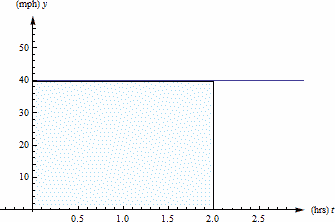
\includegraphics{images/image001.png}

To describe the values, x, that lie in the intervals shown above we
would say, ``x is a real number greater than or equal to 1 and less than
or equal to 3, or a real number greater than 5.'' As an inequality it is
``\textbackslash{}(1\textbackslash{}leq x\textbackslash{}leq
3\textbackslash{}) or \textbackslash{}(x \textbackslash{}gt 5
\textbackslash{})''. In interval notation it is
``\textbackslash{}({[}1,3{]}\textbackslash{}cup(5,\textbackslash{}infty)\textbackslash{})''.

\hypertarget{example-11}{%
\paragraph{Example 11}\label{example-11}}

Find the domain of each function:\\
a) \textbackslash{}(f(x)=2\textbackslash{}sqrt\{x+4\}\textbackslash{})\\
b)
\textbackslash{}(g(x)=\textbackslash{}dfrac\{3\}\{6-3x\}\textbackslash{})

a) Since we cannot take the square root of a negative number, we need
the inside of the square root to be non-negative.
\textbackslash{}(x+4\textbackslash{}geq 0\textbackslash{}) when
\textbackslash{}(x\textbackslash{}geq -4\textbackslash{}), so the domain
of \textbackslash{}(f(x)\textbackslash{}) is
\textbackslash{}({[}-4,\textbackslash{}infty)\textbackslash{}).

b) We cannot divide by zero, so we need the denominator to be non-zero.
\textbackslash{}(6-3x=0\textbackslash{}) when \textbackslash{}(x =
2\textbackslash{}), so we must exclude 2 from the domain. The domain of
\textbackslash{}(g(x)\textbackslash{}) is
\textbackslash{}((-\textbackslash{}infty,2)\textbackslash{}cup(2,\textbackslash{}infty)\textbackslash{}).

To view this video please enable JavaScript, and consider upgrading to a
web browser that \href{http://videojs.com/html5-video-support/}{supports
HTML5 video}

\begin{longtable}[]{@{}ll@{}}
\toprule
\endhead
\href{../index.php}{← Previous Section} & \href{section1-2.php}{Next
Section →}\tabularnewline
\bottomrule
\end{longtable}
